\documentclass[10pt, a4paper]{article} 

\usepackage[T1]{fontenc}     % We are using pdfLaTeX,
\usepackage[utf8]{inputenc}  % hence this preparation
\usepackage[british]{babel}  
\usepackage[left = 0mm, right = 0mm, top = 0mm, bottom = 0mm]{geometry}
\usepackage[stretch = 25, shrink = 25, tracking=true, letterspace=30]{microtype}  
\usepackage{graphicx}        % To insert pictures
\usepackage{xcolor}          % To add colour to the document
\usepackage{marvosym}        % Provides icons for the contact details
\usepackage{fontawesome5}

\usepackage{enumitem}        % To redefine spacing in lists
\setlist{parsep = 0pt, topsep = 0pt, partopsep = 1pt, itemsep = 1pt, leftmargin = 6mm}

\usepackage[scaled]{helvet}     % Change this to use any font, but keep it simple
\renewcommand{\familydefault}{\sfdefault}

\definecolor{cvblue}{HTML}{304263}

%%%%%%% USER COMMAND DEFINITIONS %%%%%%%%%%%%%%%%%%%%%%%%%%%
% These are the real workhorses of this template
\newcommand{\dates}[1]{\hfill\mbox{\textbf{#1}}} % Bold stuff that doesn’t got broken into lines
\newcommand{\is}{\par\vskip.3ex plus .4ex} % Item spacing
\newcommand{\smaller}[1]{{\small$\diamond$\ #1}}
\newcommand{\normal}[1]{{\normalsize$\diamond$\ #1}}
\newcommand{\headleft}[1]{\vspace*{2ex}\textsc{\textbf{#1}}\par%
	\vspace*{-1.5ex}\hrulefill\par\vspace*{0.7ex}}
\newcommand{\headright}[1]{\vspace*{2.5ex}\textsc{\Large\color{cvblue}#1}\par%
	\vspace*{-2ex}{\color{cvblue}\hrulefill}\par}
%%%%%%%%%%%%%%%%%%%%%%%%%%%%%%%%%%%%%%%%%%%%%%%%%%%%%%%%%%%%

\usepackage[colorlinks = true, urlcolor = white, linkcolor = white]{hyperref}

\begin{document}
	
	% Style definitions -- killing the unnecessary space and adding the skips explicitly
	\setlength{\topskip}{0pt}
	\setlength{\parindent}{0pt}
	\setlength{\parskip}{0pt}
	\setlength{\fboxsep}{0pt}
	\pagestyle{empty}
	\raggedbottom
	
	\begin{minipage}[t]{0.33\textwidth} %% Left column -- outer definition
		%  Left column -- top dark rectangle
		\colorbox{cvblue!90}{\color{white}  %% LEFT BOX
			\kern0.09\textwidth\relax% Left margin provided explicitly
			\begin{minipage}[t][297mm][t]{0.82\textwidth}
				\raggedright
				\vspace*{2ex} % Extra space after the picture
				% Centering without extra vertical spacing
				\null\hfill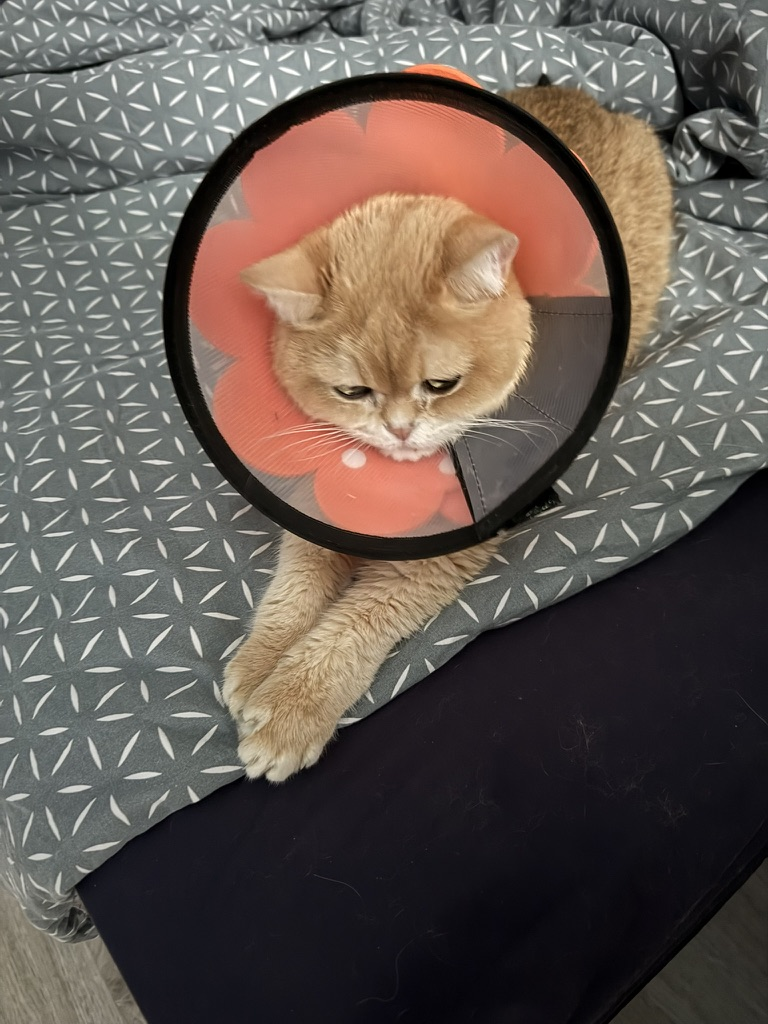
\includegraphics[height=0.85\textwidth]{avatar.jpg}\hfill\null

				
				\vspace*{1.5ex}
				
				\Large  \textbf{Vladislav Metel} \normalsize 
				
				\vspace*{1.5ex}
				
				Expert SDET | AWS Automation | Python | CI/CD Architect | LLM-Enhanced QA
				
				\headleft{Contact details}
				
				\begin{tabular}{ @{}c l }
					\Letter\ & \href{mailto:metel.vlad@gmail.com?subject=Job Opportunity}{metel.vlad@gmail.com} \\
					\faLinkedin\ & \href{https://www.linkedin.com/in/metelvladislav}{metelvladislav} \\
					\faMobile*\ & \href{tel:+7 999 825 23 92}{\raisebox{0.2ex}{+}7 999 825 23 92} \\
					\faGithub\ & \href{https://github.com/IamVladislav}{IamVladislav} \\
				\end{tabular}
				
				\headleft{Languages}
				Russian: \textbf{Native} \\[2pt]
				English: \textbf{Upper intermediate} \\[2pt]
				Spanish: \textbf{Pre-intermediate}
				
				
				\headleft{Skills}
				\normal{Languages: \textbf{Python, TypeScript, Bash}} \\[1pt]
				\normal{AWS Cloud: \textbf{CloudFormation, Lambda, DynamoDB, EC2, ECS, API Gateway, CloudFront, VPC}} \\[1pt]
				\normal{ML/LLM: \textbf{AWS Bedrock (Anthropic Claude, AWS Nova), SageMaker/HuggingFace (Qwen), PyTorch, OpenCV}} \\[1pt]
				\normal{CI/CD: \textbf{Bitbucket/Bamboo, GitHub/GithubActions}} \\[1pt]
				\normal{Mix: \textbf{Docker, Docker Compose}} \\[1pt]
				\normal{Testing: \textbf{PyTest, Mock Systems, Screenshot/CV testing, Selenium}}
				
								
				\headleft{Certifications/Pet Projects}
				\textbf{AWS Certified Solutions Architect – Associate} \\[1pt]
				\textbf{\href{https://github.com/IamVladislav/pytest-mitmproxy-plugin}{MITMProxy plugin for pyTest}}
			\end{minipage}%
			\kern0.09\textwidth\relax%%Right margin provided explicitly to stretch the colourbox
		}
	\end{minipage}% Right column
	\hskip2.5em% Left margin for the white area
	\begin{minipage}[t]{0.56\textwidth}
		\setlength{\parskip}{0.5ex}% Adds spaces between paragraphs; use \\ to add new lines without this space. Shrink this amount to fit more data vertically
		
		\headright{Summary}
		
		Innovative SDET with 7+ years of experience in building large-scale, AWS-based automation systems for QA. Proven track record in reducing testing costs by over 60\% through dynamic test selection, ML-based analysis, and scalable CI/CD infrastructure. Passionate about leveraging cloud-native architectures, LLMs, and DevOps practices to improve software quality and engineering velocity. Experienced team leader and mentor with a strong Python and infrastructure-as-code background.
		
		
		
		\headright{Experience}
		
		\textsc{Expert SDET} at \textit{Align Technology}  \dates{March 2021 – Present}
		
		\textbf{Scalable Infrastructure \& Cloud Automation}
		\is
		\smaller{Built and maintained a highly scalable test execution infrastructure on AWS, automating the provisioning and lifecycle management of thousands of on-demand workers to support the execution of 5M+ UI tests per week}
		\is
		\smaller{Architected a region distribution algorithm to automatically balance load between regions based on current Spot price and availability, after introducing the system, spot instance errors were eliminated while maintaining low costs}
		\is
		\smaller{Implemented a multi-regional, performance-aware upload system to Allure TestOps with auto-switching based on cluster load, reducing performance degradation and enabling in-process uploads for 70\% of test runs}
		
		\textbf{CI/CD Optimization \& DevOps Tooling}
		\is
		\smaller{Engineered and rolled out a custom CI toolkit across 10 AQA teams, standardizing pipelines and improving consistency within the unit}
		\is
		\smaller{Developed a React-based portal for test artifact management, integrating multi-regional S3 storage, AWS Lambda pipelines, and AWS Cognito + Azure AD for secure authorization}
		
		\textbf{Smart Automation \& ML/LLM Integration}
		
		\is
		\smaller{Designed and implemented AI review system based on AWS Stack via Bedrock and SageMaker models, using a custom context extractor powered by AWS Lambda and providing useful comments in 5 minutes after pull request creation}
	
		\is
		\smaller{Implemented a change-based test selection mechanism, optimizing test execution by running only the tests impacted by code changes, resulting in a 30\% ( ~300k\$ annually ) reduction in testing costs}
		
		\is
		\smaller{Introduced a time-optimized test session framework with dynamic per-test timeouts, significantly improving the efficiency and speed of the testing process, leading to an additional 20\% ( ~100k\$ annually ) cost savings}
		
		\is
		\smaller{Built a custom test stability detection mechanism that dynamically determines the need for retries, improving test reliability and reducing false failures, which increased the overall success rate from 70\% to 99\%}
		
		\is
		\smaller{Trained and integrated neural network for object segmentation and detecting elements on WebGL scene via PyTorch and openCV}
		
		\is
		\smaller{Refactored test framework - introduced independent fixtures and plug-ins to collect logs and results, mentoring teammates, helped increase the number of tests from 5k to 18k+}
		
		\textbf{Mock Systems \& Environment Virtualization}

		\is
		\smaller{Implemented mock system, based on AWS (Lambda, S3, DynamoDB, API Gateway, CloudFront), Docker and Python (aiohttp, flask), which raised the success rate from 40\% to 70\% while enabling one-click state viewing from a browser}
		
		\textbf{Leadership \& Collaboration}
		
		\is
		\smaller{Managed a team of up to 4 SDETs, providing leadership and guidance in the development and enhancement of internal testing systems}
		
		
	\end{minipage}
	
	\newpage
	\vspace*{2ex}
	\hskip0.05\textwidth% Left margin for the white area
	\begin{minipage}[t]{0.9\textwidth}
		\setlength{\parskip}{0.5ex}% Adds spaces between paragraphs; use \\ to add new lines without this space. Shrink this amount to fit more data vertically
		
		\headright{Experience}
		
		\textsc{QA Engineer} at \textit{VK ex. Mail.Ru Group}  \dates{May 2018 – March 2021}
		
		\textbf{Automation testing}
		\is
		\smaller{Designed and implemented a desktop automation framework from scratch using a custom driver based on the Qt internal testing API}
		\is
		\smaller{Scaled the number of automated tests from 100 to over 1,000}
		\is
		\smaller{Developed guidelines and a foundation enabling developers to contribute to automated tests as part of the development lifecycle}
		
		\textbf{Infrastructure}
		\is
		\smaller{Built and maintained a cross-platform testing environment for release smoke testing using a combination of supported systems on VMware}
		\is
		\smaller{Set up automation bots for test progress reporting and assigning duties to responsible team members}
		
		\textbf{Manual testing \& Team}
		\is
		\smaller{Actively participated through the development process starting from the design and idea to release}
		\is
		\smaller{Mentored junior colleagues and reviewed implemented features}
		\is
		\smaller{Advocated for unified testing tools across teams led the transition to Charles Proxy and Postman for API testing, enabling QA engineers to seamlessly switch between teams without learning new tools}
		\par{\color{cvblue}\hrulefill}\par
		\textsc{Engineer} at \textit{Russian Academy of Sciences | RAS · Institute of Crystallography}  \dates{Febriary 2017 – April 2019}
		
		\textbf{Development}
		\is
		\smaller{Developed a C++ project to simulate diffraction patterns of distorted crystals}
		\is
		\smaller{Used cluster computing to parallelize execution across hundreds of processes, reducing simulation time from several days to hours}
		
		\headright{Education}
		\vspace*{1ex}
		\textbf{Master of Science in Applied Mathematics and Computer Science} \\[1pt]
		\vspace*{1ex} %Why?
		\small
		NRNU MEPhI (National Research Nuclear University MEPhI), 2017–2019 \\[1pt]
		\normalsize
		\textbf{Bachelor of Science in Applied Mathematics and Computer Science} \\[1pt]
		\small
		NRNU MEPhI (National Research Nuclear University MEPhI), 2013–2017 \\[1pt]
		\normalsize

	\end{minipage}
	
	
\end{document}